% !TEX root = ../main.tex

\chapter{Machine learning basics}
\label{ch:mlbasics}
This chapter highlights and explains the machine learning basics to understand the Hydra framework. First, a little overview and history of machine learning is shown. Then, the supervised learning paradigm is explained, by introducing some mathematical concepts, such as loss functions. After that, the applications and the basics of neural networks are presented. Deep learning will then quickly be introduced, to finally come to well known convolutional networks, that are used in computer vision and for a computer aided diagnosis applications. When having all this solid mathematical and conceptual background, the Hydra framework will finally be understandable, and presented in the last section.

\section{Overview}
\label{sec:mloverview}
Machine learning uses algorithms to learn about given data, and improves on finding solutions to a problem\footnote{\url{https://www.ibm.com/cloud/learn/machine-learning}}. Solutions in machine learning consist of trained mathematical models, generic functions accompanied with a parameter set. Machine learning assumes that for each given dataset, there is an \emph{underlying function} that generates the data. The goal of machine learning algorithms is then to find a solution that best fits the data, and that is the closest to the real underlying function, by learning through the data. Solutions are always \emph{approximations} of the real underlying function, limited by the data the machine knows, or that the user gives to it, which is only a subset of the whole possible data. After this period of learning, many applications can be done. Prediction, classification, clustering and anomaly detection can be cited as some of the most used generic applications of machine learning.

Machine learning has first started back in the 1950's. Firstly, the statistical methods or main concepts of machine learning were created, as in the work of \citet{hebb_organization_2002}, who based his work in the synaptic transmission of signals of electrical impulses, that will be used further in neural networks. In 1957, one of the fundamental algorithm of machine learning, the perceptron, was invented by \citet{rosenblatt_perceptron_1958}, who published his work in 1958. The perceptron is a binary classifier algorithm, that is at the very base of all neural networks. Further, in 1963, \citet{michie_boxes_1968} developed a machine made of matchboxes that learns how to play Tic-Tac-Toe and plays against humans. The machine makes a decision move depending on the current position of the boardgame. A turning point in the history of the machine learning was back in 1988, when \citet{lecun_theoretical_1988} published their work about the backpropagation algorithm, that is still used today to train neural networks.

Today, machine learning has a plenty of real world applications, such as email spam detection, recommender systems, face recognition, or language translators, to only cite them. Machine learning is comprised of three main paradigms, that have different behaviour and can be choosen depending on the problem that needs to be solved\footnote{\url{https://towardsdatascience.com/what-is-machine-learning-891f23e848da}}. These paradigms are:

\vbox{
  \begin{enumerate}
    \item Supervised learning
    \item Unsupervised learning
    \item Reinforcement learning
  \end{enumerate}}

Figure~\ref{fig:paradigms} shows the three main paradigms and some of their applications. The rest of the work will focus on the supervised learning paradigm, which is explained in detail next.

\begin{figure}[t!]
  \centering
  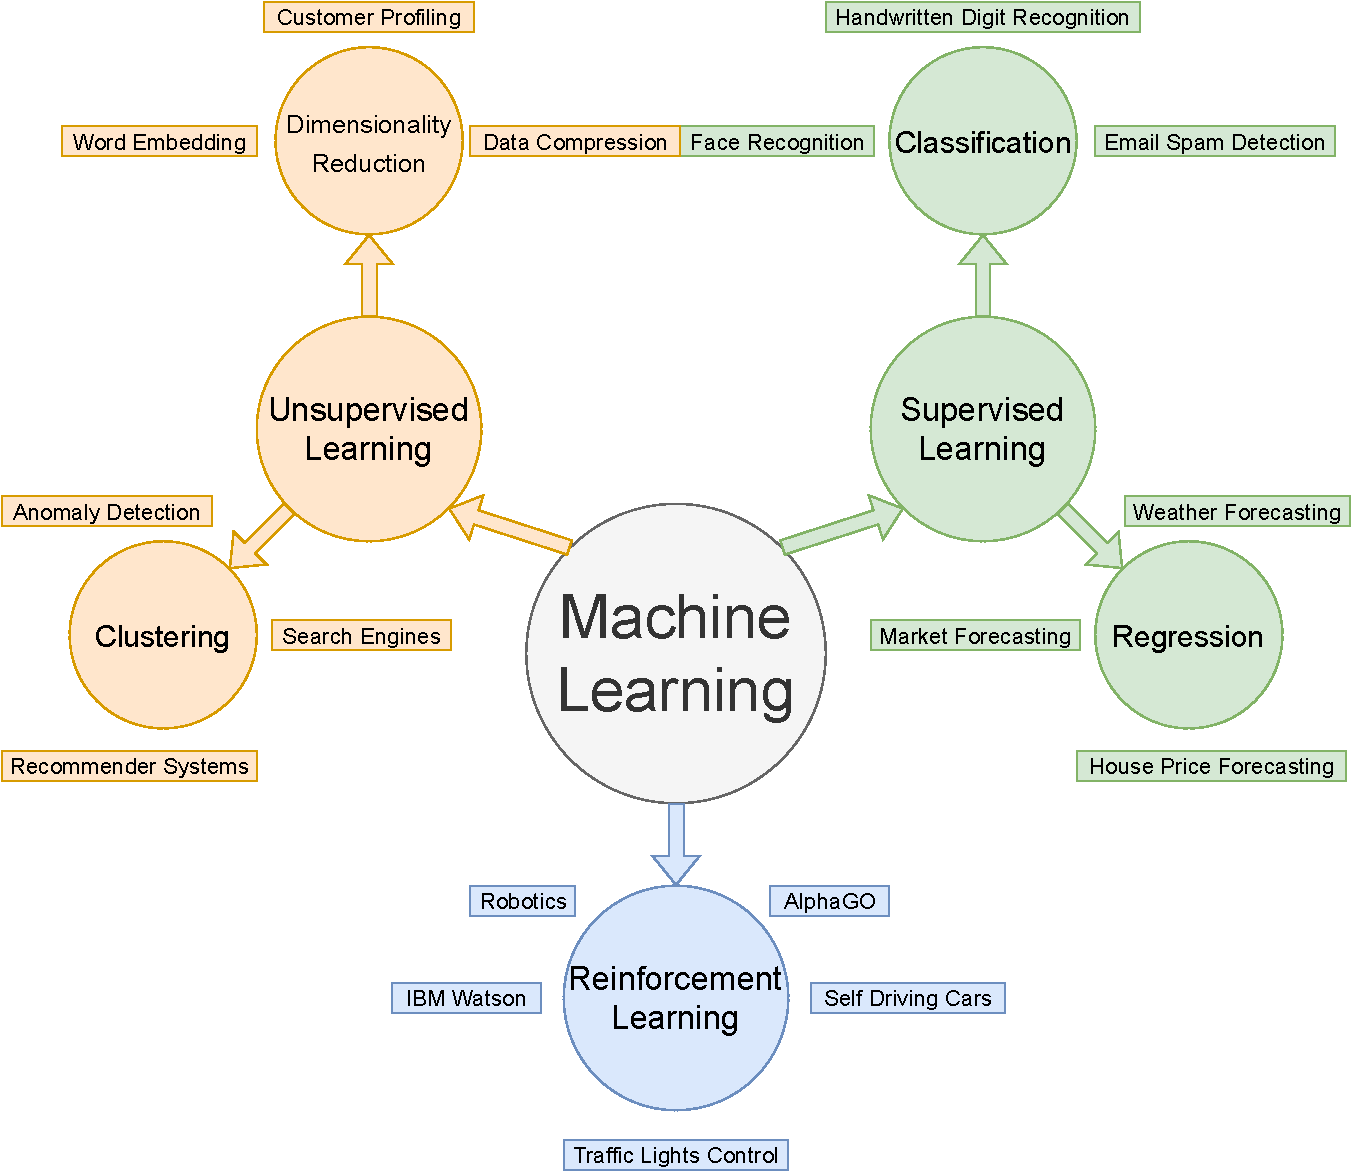
\includegraphics[width=\textwidth]{mlbasics/mlparadigms.pdf}
  \caption[Machine learning main paradigms]{Some applications of the three main machine learning paradigms.}
  \label{fig:paradigms}
\end{figure}


\section{Supervised learning}
\label{sec:sl}
As its name suggests, the learning is done in a supervised manner, like a teacher will supervise his students. To be used, supervised learning algorithms need a set of data, called the \emph{training dataset}, i.e. the data from which the underlying function is learned. The training data is composed of tuples of two elements. The first element is an input/entry element, and the second is the known answer corresponding to the input element, called the \emph{label}\footnote{\url{https://deepai.org/machine-learning-glossary-and-terms/supervised-learning}}. The goal of supervised learning algorithms is to find the relation between the input data and their corresponding labels, or in mathematical terms, to find the underlying function $f: X \to Y$ such as:
\begin{equation}
  f(x) = y
\end{equation}
where $x \in X$ is an element of the input space $X$ and $y \in Y$ its corresponding label in the decision space $Y$. The so called training dataset $D$ is then a set of tuples containing an element $x_i$ of the input space with its corresponding label $y_i$, so mathematically $D = \{(x_i, y_i), i \in \{1, ..., n\}\}$. To best approximate $f$, i.e. to learn from the training data, the algorithm starts with a solution $h_1$, and constructs a prediction $\hat{y}$ based on the input $x$, such as:
\begin{equation}
  h_1(x) = \hat{y}
\end{equation}
Then, it compares the true label $y$ with the prediction $\hat{y}$. Depending on this comparison, the algorithm modifies a bit the solution $h_1$ into the improved solution $h_2$. This process is iterated, and the solution is improved and will approximate better and better the true underlying function $f$. The quality of the prediction of the model is verified by using \emph{loss functions}.

\subsection{Loss functions}
A loss function estimates the cost or severity of predicting the actual prediction $h(x_i) = \hat{y}_i$ rather than the real value $y_i$. With that information, the algorithm knows if it is improving in a good direction, and have an idea how to minimze this loss. There are many loss functions that have different form, and that are more or less representative on specific applications. Given a training data point $(x_i, y_i)$ and a model $h$ to train, here are some often used loss function examples. Firstly, the \emph{squared error loss} is given by:
\begin{equation}
\label{eq:squaredloss}
  L(h(x_i), y_i) = (y_i - h(x_i))^2
\end{equation}
This is one of the simpliest and most used loss function for a regression problem. A small variation of this loss function that is often used is to add a factor $\frac{1}{2}$ to simplify computing the derivative. As second example loss function, the \emph{hinge loss} is used for binary classification, by penalizing the wrong prediction, but also the right ones that are not confident. It has the form:
\begin{equation}
  L(h(x_i), y_i) = \text{max} (0, 1 - y_i \cdot h(x_i))
\end{equation}
Finally, a similar loss function to the first loss function~\eqref{eq:squaredloss} is the \emph{absolute error loss}, given by:
\begin{equation}
  L(h(x_i), y_i) = |y_i - h(x_i)|
\end{equation}
This third loss function is more robust than the squared error because it is generally not affected by outliers. But on the other side, the squared error tends to adapt the model regarding the outliers. The loss function gives the information about how bad or good is one prediction. For an entire training dataset, the sum of the losses of all points in the dataset is required and will be more representative. This sum is called the \emph{empirical risk}, and will be used also further to tune neural networks. The empirical risk is given by:
\begin{equation}
  \hat{R}(h) = \sum^n_{i=1} L(h(x_i),y_i)
\end{equation}
The empirical risk can be averaged by a factor $\frac{1}{n}$ in certain cases, for example with the backpropagation algorithm (see further in Section~\ref{sec:backprop}).

A key point in the training phase is not to learn too much from the given data. Indeed, as stated in introduction of this chapter, the training data is only a subset of the real whole data. When the algorithm learns the available data too closely, it specializes on this precise data and is not able to predict well the future unseen data, resulting in a bad generalization. This phenomenon is called \emph{overfitting}.

Finally, supervised learning is mainly used for classification or regression problems, and is one of the most used paradigms in machine learning. A class of algorithm that are very strong with supervised learning are neural networks. In the following section, neural networks will be presented in detail.

\section{Neural Networks}
Nowadays, an extremely important concept that is used in machine learning is the \emph{neural network}. Neural networks are inspired by biological brains, that connect neurons with synapses. The concept of the natural neural network and the artificial neural network is to pass some information by connections. Neural networks are commonly trained using supervised learning. Figure~\ref{fig:neuron} shows the form of an artificial neuron, in comparison with biological neuron technical terms.
\begin{figure}[t!]
  \centering
  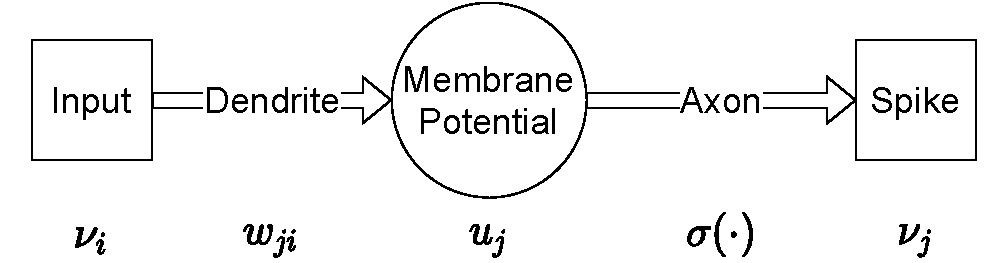
\includegraphics[width=\textwidth]{mlbasics/neuron.pdf}
  \caption[Schema of an artificial neuron]{Schema showing how an artificial neuron works. The input $\nu_i$ of the neuron is first weighted by some weight $w_{ji}$ that represents the connection beetween $i$ and $j$. The result is the membrane potential $u_j$, that is finally activated by an activation function $\sigma(\cdot)$. The output of the neuron is given by $\nu_j$.}
  \label{fig:neuron}
\end{figure}

An artifical neural network is composed of many neurons distributed in \emph{layers}. A neural network can have a variable number of layers depending on the task. Each layer is more or less connected to each other by neurons. Different shape of connections make different type of neural network. In each layer, there is one or several neurons. Each neuron has one or more inputs, that are the output of the neurons of the previous layer, but only one output. The neuron will take its inputs, arrange them according learned weights, and activate using an \emph{activation function}, and finally give the output. Mathematically, this is represented by the following formulas:
\begin{align}
  \begin{split}
    u_j &= \sum^k_{i=1} w_{ji} \cdot \nu_i \\
    \nu_j &= \sigma(u_j)
  \end{split}
\end{align}
where $u_j$ is the membrane potential of the neuron, $\nu_i$ are the inputs of the previous layer, $w_{ji}$ the synaptic weight of the neuron of the connection $i$ to $j$, and $\nu_j$ the output of the neuron, after activation with $\sigma(\cdot)$. There are several activation functions that can be used, for example the \emph{logistic} function:
\begin{equation}
  \sigma(x) = \frac{1}{1 + e^{-x}}
\end{equation}
As second example, the \emph{hyperbolic tangent}:
\begin{equation}
  \sigma(x) = \text{tanh}(x) = \frac{2}{1 + e^{-2x}} - 1
\end{equation}
Or the \emph{rectified linear unit} (ReLU) function:
\begin{equation}
  \label{eq:relu}
  \sigma(x) = \begin{cases}
    0 & \text{if } x < 0 \\
    x & \text{if } x \geq 0
  \end{cases}
\end{equation}
And at last example, the \emph{exponential linear unit} (ELU):
\begin{equation}
  \label{eq:elu}
  \sigma(x) = \begin{cases}
    \alpha (e^{x} - 1) & \text{if } x < 0 \\
    x & \text{if } x \geq 0
  \end{cases}
\end{equation}
These activation functions are again choosen depending on the task the neural network needs to do. For example, the logistic function will be more used for a binary classification task, as its output range is from 0 to 1, and can represent a probability. Compared to this, the hyperbolic tangent has the advantage to have an output range from -1 to 1. The two other examples, the ReLU and ELU are some of the most common choices in deep learning and convolutional networks. Both have their output range that goes towards infinity, but they differ in the lower bound. ReLU puts its negative values to zero immediately, whereas ELU will have a lower bound equal to $\alpha$. ELU has so the advantage to treat smoothly the negative values but at the cost to be slower to compute than the ReLU\footnote{\url{https://towardsdatascience.com/activation-functions-neural-networks-1cbd9f8d91d6}}.

The functioning of a neural network is the following. An input is given to the network, and it goes through several layers inside the network. At each layer, more or less outputs go out, and enter the next layer. At the other side of the network, in the last layer, the output of the network goes out, and is the final output, given the very first input. The output can have a very different form regarding the task that has to be achieved. For example, if a neural network is constructed to recognize if there is a cat in an image, then the input will be an image, and the output will be a binary output, with probabilities of true (there is a cat) or false (there is no cat).

Figure~\ref{fig:neuralnetwork} represents a neural network with two inputs $x_1$ and $x_2$, one hidden layer of two neurons $n_1$ and $n_2$, and one output layer of one neuron $n_3$. The weights are represented as $w_{ji}$. The computations inside the network go as follows. First, the weights are putting in a weight matrix, one matrix between each layer. The matrix between the inputs and the hidden layer is $W_{in}$, as the matrix between the hidden layer and the ouput layer is $W_{hid}$. Then, the inputs are stored in a vector $x$, the intermediate results are in the vector $n_{hid}$ and the output in $n_{out}$. The activation function in each neuron is $\sigma(\cdot)$. These definitions are given by:
\begin{align}
  \begin{split}
    W_{in} = \begin{pmatrix}
      w_{11} && w_{12}\\
      w_{21} && w_{22}
    \end{pmatrix}, \hspace{0.8cm}
    W_{hid} = \begin{pmatrix}
      w_{31} && w_{32}
    \end{pmatrix} \\
    x = \begin{pmatrix}
      x_1\\ x_2
    \end{pmatrix}, \hspace{0.8cm}
    n_{hid} = \begin{pmatrix}
      n_1\\ n_2
    \end{pmatrix}, \hspace{0.8cm}
    n_{out} = \begin{pmatrix}
      n_3
    \end{pmatrix}
  \end{split}
\end{align}
With the help of these definitions, the formulas to compute the intermediate results can be written using matrices multiplication from linear algebra:
\begin{align}
  \begin{split}
    n_{hid} &= \sigma(W_{in}x) = \begin{pmatrix}
      \sigma(w_{11} x_1 + w_{12} x_2)
      \sigma(w_{21} x_1 + w_{22} x_2)
    \end{pmatrix} \\
    n_{out} &= \sigma(W_{in} n_{hid}) = \begin{pmatrix}
      \sigma(w_{31} n_1 + w_{32} n_2)
    \end{pmatrix}
  \end{split}
\end{align}
And the full equation for the output of the example network can be written using the two equations above:
\begin{equation}
  \text{out} = n_3 = \sigma(w_{31} \sigma(w_{11} x_1 + w_{12} x_2) + w_{32} \sigma(w_{21} x_1 + w_{22} x_2))
\end{equation}

\begin{figure}[t!]
  \centering
  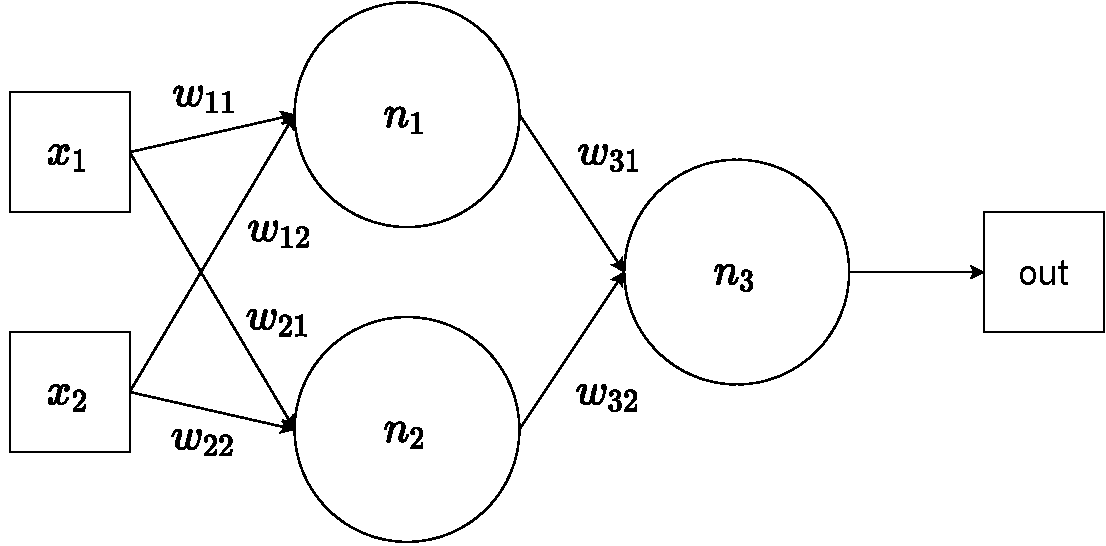
\includegraphics[width=\textwidth]{mlbasics/neuralnetwork.pdf}
  \caption[Neural network example]{Schema representing an example neural network. It contains one hidden layer of two neurons $n_1$ and $n_2$, and one output layer of one neuron $n_3$. $x_1$ and $x_2$ are the two inputs of the network, whereas the neuron $n_3$ gives the output of the network. The $w_{ji}$ are the six weights.}
  \label{fig:neuralnetwork}
\end{figure}

Mathematically speaking, a neural network is an universal function approximator. That means that a neural network can approximate any function from a theoretical perspective. In that way, neural networks can be used for quite any applications, given a network large enough. Neural networks are parametrized by their structure, i.e. how the layers are disposed, their activation functions and their weights. Different values for the weights can lead to very different outputs, thus the weights need to be well tuned. To give values to the weights in an optimal manner, a well-known algorithm is used: the \emph{backpropagation}. This is the main algorithm to train the network and to tune its weights, in the way to do a specific application.

\section{Backpropagation}
\label{sec:backprop}
As stated in Section~\ref{sec:mloverview}, the backpropagation was invented in the end of the 1980's, by simultaneous works of different researchers. The backpropagation algorithm is used with neural networks, and will adapt or optimize the weights of the network. Backpropagation is composed of two phases. The first one is called the \emph{forward pass}, when the inputs are propagating from the front of the network to the back, i.e. the network makes a prediction. Then, the prediction is compared to the ground truth label, and the error is computed with a loss function. In the second phase called the \emph{backward pass}, the error is propagating from the back of the network to the front. For each layer, the derivative of the error is computed. These derivatives help to know which weights contributed to the error, and help adapting them in a focused manner.

For a network, the backpropagation algorithm computes the error as the risk over all points of the dataset. The error depends on the weights set $w$ of the network. Indeed, different weights lead to different predictions, thus different errors. Let the error $E(w)$ of the network be:
\begin{equation}
  \label{eq:generalerrfun}
  E(w) = \frac{1}{|S|}\sum_{i \in S} L(f_w(x_i), y_i)
\end{equation}
with $f_w(\cdot)$ the function representing the network with specific weights $w$, $L(\cdot, \cdot)$ a choosen loss function, and $S$ a sample of the training data. This sample $S$ can be different regarding the type of training that is made. For example, $S$ can be the whole training dataset and the training is called to be in batch mode. In contrast, the sample can be choosen to be $|S| = 1$, that is called in online mode. But the most common way to train nowadays is the so called mini batches, by choosing $|S| \ll n$, that is in a small subset at each step of the learning. In general for backpropagation, the loss function used is the squared loss~\eqref{eq:squaredloss} with a $\frac{1}{2}$ factor. The error function~\eqref{eq:generalerrfun} for backpropagation will then be:
\begin{equation}
  \label{eq:backerrorfunction}
  E(w) = \frac{1}{2|S|}\sum_{i \in S} (f_w(x_i) - y_i)^2
\end{equation}

Note that in the following paragraphs and formulas, the symbols in superscript within parenthesis will represent the number of the current layer, as the symbols in subscript will represent the number of the neuron it refers. As example, the notation $\nu^{(l)}_n$ will refer to the output after activation of the $n$-th neuron of the layer $l$.

The goal of the backpropagation is to minimize the error function~\eqref{eq:backerrorfunction} of the network, to make the network as strong as possible in its predictions. To do that, weights must be tuned and adapted to make the best results. To know in which direction the weights must be changed regarding the error, backpropagation uses \emph{gradient descent}. This method iteratively finds a local mimimum or maximum of a differentiable function. In this method, the gradient of the increasing error is $\nabla_w E(w)$, and so the direction of the decreasing error will be in the opposite direction of the gradient, i.e in $-\nabla_w E(w)$ direction. A learning rule for a single weight can then be derived as:
\begin{equation}
  w^{(k)}_{ji} \gets w^{(k)}_{ji} - \eta \cdot \nabla_w E(w)
\end{equation}
where $\eta$ is called the learning rate. This rule shows that the weights are updated regarding the most decreasing error direction. As the error function $E(w)$ is differentiable with respect to the weights $w$, gradient descent can be applied and that is what backpropagation does. Mathematically\footnote{\url{https://brilliant.org/wiki/backpropagation/}}, the error gradient with the weight for neuron $j$ in layer $k$ connected to incoming neuron $i$ of previous layer is defined as:
\begin{equation}
  \nabla_w E(w) = \frac{\partial E}{\partial w^{(k)}_{ji}}
\end{equation}
Remember that in Figure~\ref{fig:neuron}, $u_j^{(k)}$ was denoted to be the membrane potential of neuron $j$ in the layer $k$, that is the value before going in the activation function. Let $n^{(k)}$ defines the number of neuron in the layer $k$, $u_j^{(k)}$ is computed by the sum:
\begin{equation}
  \label{eq:layeroutput}
  u_j^{(k)} = \sum^{n^{(k-1)}}_{m=1} w^{(k)}_{jm} \nu^{(k-1)}_m
\end{equation}
The partial derivative of the error with respect to one weight is computed using the chain rule, and is then given by:
\begin{equation}
  \label{eq:errorgradient}
  \frac{\partial E}{\partial w^{(k)}_{ji}} = \frac{\partial E}{\partial u_j^{(k)}} \frac{\partial u_j^{(k)}}{\partial w^{(k)}_{ji}}
\end{equation}
The first term of~\eqref{eq:errorgradient} is in general called the backpropagated error, and is written as:
\begin{equation}
  \label{eq:errorterm}
  \delta_j^{(k)} = \frac{\partial E}{\partial u_j^{(k)}}
\end{equation}
Whereas the second term is calculated to be $\nu_i^{(k-1)}$ the output after the activation of the neuron $i$ in the layer $k-1$, i.e. the previous layer:
\begin{equation}
  \frac{\partial u_j^{(k)}}{\partial w^{(k)}_{ji}} = \frac{\partial}{\partial w^{(k)}_{ji}} \left( \sum^{n^{(k-1)}}_{m=1} w^{(k)}_{jm} \nu^{(k-1)}_m \right) = \nu_i^{(k-1)}
\end{equation}
In summary, the derivative of the error~\eqref{eq:errorgradient} regarding a weight can be written in the compact form:
\begin{equation}
  \label{eq:errorcompact}
  \frac{\partial E}{\partial w^{(k)}_{ji}} = \delta_j^{(k)} \nu_i^{(k-1)}
\end{equation}

On one hand, for the output layer $l$, i.e. the last layer of the network, \eqref{eq:errorcompact} will depend directly on the label $y$ and the prediction $f_w(y)$. By applying the chain rule and using the derivative of~\eqref{eq:backerrorfunction}, the derivative of the error that is~\eqref{eq:errorcompact} will become:
\begin{equation}
  \frac{\partial E}{\partial w^{(l)}_{ji}} = \delta_j^{(l)} \nu_i^{(l-1)} = (f_w(y) - y) \cdot \sigma'\left( \sum^{n^{(k-1)}}_{m=1} w^{(l)}_{jm} \nu^{(l-1)}_m \right) \cdot \nu_i^{(l-1)}
\end{equation}
On the other hand, for a hidden layer $k$, the error term~\eqref{eq:errorterm} is first computed by again using the chain rule:
\begin{equation}
  \delta^{(k)}_j = \frac{\partial E}{\partial u_j^{(k)}} = \sum^{n^{(k+1)}}_{m=1} \frac{\partial E}{\partial u_m^{(k+1)}} \frac{\partial u_m^{(k+1)}}{u_j^{(k)}}
\end{equation}
But the first term in this sum represents also an error term~\eqref{eq:errorterm}. By using the definition and derivative of~\eqref{eq:layeroutput}, the error term for hidden layers will become:
\begin{equation}
  \label{eq:hidlayerror}
  \delta^{(k)}_j = \sum^{n^{(k+1)}}_{m=1} \delta^{(k+1)}_m \cdot w^{(k+1)}_{jm} \cdot \sigma'(u^{(k)}_j)
\end{equation}
Finally, by taking the result of~\eqref{eq:hidlayerror}, the derivative of the error~\eqref{eq:errorcompact} for hidden layers will be:
\begin{equation}
  \frac{\partial E}{\partial w^{(k)}_{ji}} = \sigma'(u^{(k)}_j) \cdot \nu_i^{(k-1)} \cdot \sum^{n^{(k+1)}}_{m=1} \delta^{(k+1)}_m \cdot w^{(k+1)}_{jm}
\end{equation}
This last equation shows that the error at layer $k$ is also depending on the error at layer $k+1$, that means that the computations of these errors must be done backwards. That is where the backpropagation algorithm takes its name. Figure~\ref{fig:backprop} shows the two steps of the backpropagation: the forward pass where the prediction is made, and the backward pass where the errors are computed.
\begin{figure}[t!]
  \centering
  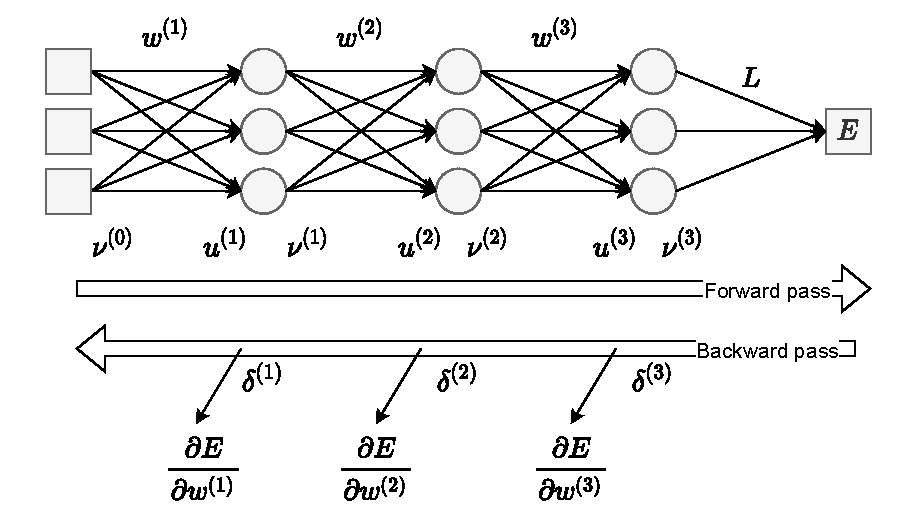
\includegraphics[width=\textwidth]{mlbasics/backprop.pdf}
  \caption[Backpropagation algorithm schema]{Schema representing the backpropagation algorithm steps. First, the forward pass is done, where the input $\nu^{(0)}$ go through the network, generating an output prediction. This prediction $\nu^{(3)}$ is compared with the actual target label, and the error $E$ is computed using the loss $L$. During the backward pass, the errors $\delta^{(i)}$ are computed, and used in the calculation of the partial derivatives. This derivatives help to adjust the weights $w^{(i)}$ of the neural network.}
  \label{fig:backprop}
\end{figure}

\section{Deep learning}
\label{sec:deeplearning}
In the recent years, some of the best results of the field come from \emph{deep learning}. Deep learning is a learning technique that uses a neural network containing many layers. That makes the network, as the name suggests, a deep network. Deep learning starts to appear in the 2010's. Before that time, it was not possible to develop deep learning. Main factors that have helped the development of deep learning were the multilayers neural networks, \emph{big data}, and the power of computations of the machines that are now enough strong to compute deep learning algorithms. The foundation of deep learning is contained in the work of \citet{goodfellow_deep_2016}, that was published in 2016.

Deep learning is used in many applications such as translators, image processing, natural language processing, and others. A major problem with deep learning however, is that the deep networks need a lot of data to be trained, which is not always easy to obtain. For example, in medical applications, the privacy of the patients data makes it difficult to collect enough data to use with deep learning. Indeed, personal information of the patients are sensible, and hence must be removed before giving public access to the data, as in the Cancer Imaging Archive.

\subsection{Convolutional neural networks}
From image classification to object detection, computer vision is used in different applications such as face recognition, autonomous cars or for military purpose. One of the most popular neural network model used for computer vision is the \emph{convolutional neural network} (CNN). One of the first CNN was when \citet{lecun_backpropagation_1989} used backpropagation to recognize handwritten zip codes. Convolutional neural networks take an image as input, and can do several tasks, such as classification, localization or segmentation (see Section~\ref{sec:tasks}).

The general structure of a convolutional neural network is composed of a first part called \emph{feature extractor} or feature learning part, that is a combination alternating \emph{convolutional layers} and \emph{pooling layers}. The second part is one or more fully connected layers that is a \emph{decision maker}. Figure~\ref{fig:cnn} shows the general architecture of a CNN.

\begin{figure}[t]
  \centering
  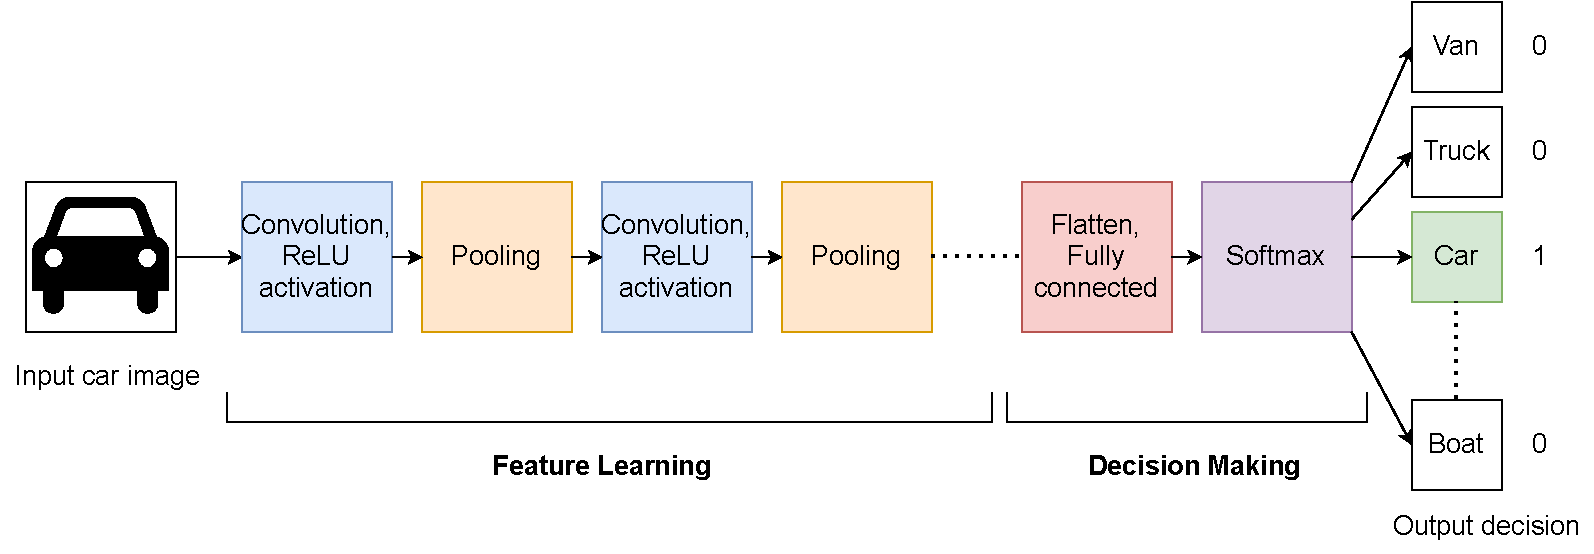
\includegraphics[width=0.96\textwidth]{mlbasics/cnn.pdf}
  \caption[Architecture of a convolutional neural network]{General architecture of a convolutional neural network. The first part represents a feature extractor, that analyzes the input image by several convolutions and poolings to extract features. These features are fed to the second part, that is a decision maker. In this example, the decision maker is a multi-class classifier that will output the probability that the image is a given vehicle, with the help of the last softmax layer that outputs a vector of probability to be in a given class.}
  \label{fig:cnn}
\end{figure}

To extact features of an image, CNNs alternate convolutions and poolings. Convolution is a mathematical operation between two objects that indicates correlated features of these objects. In computer vision, the two objects used in a convolution are the input image itself and a \emph{kernel} or \emph{mask}. A kernel is a two dimensional matrix. The form and the values of the kernel will define the effect of the convolution when applied to the image. For example, kernels can detect ridges, vertical or horizontal lines, or sharp the image. To perform a convolution, a window (subarea of the image) containing the kernel values will slide over the image iteratively. At each step, a convolved feature is outputed. Convolutions are characterized by parameters such as the size of the kernel, the stride i.e. by how much the window is moved in a single iteration, and paddings that can add pixel in the border of the image. Depending on these parameters, the outputed convolved features can have the same size, or a reduced dimensionality compared to the input image. Figure~\ref{fig:convolution} shows 4 steps during a convolution, that applies an element-wise multiplication between the image and the kernel.

\begin{figure}[t]
  \centering
  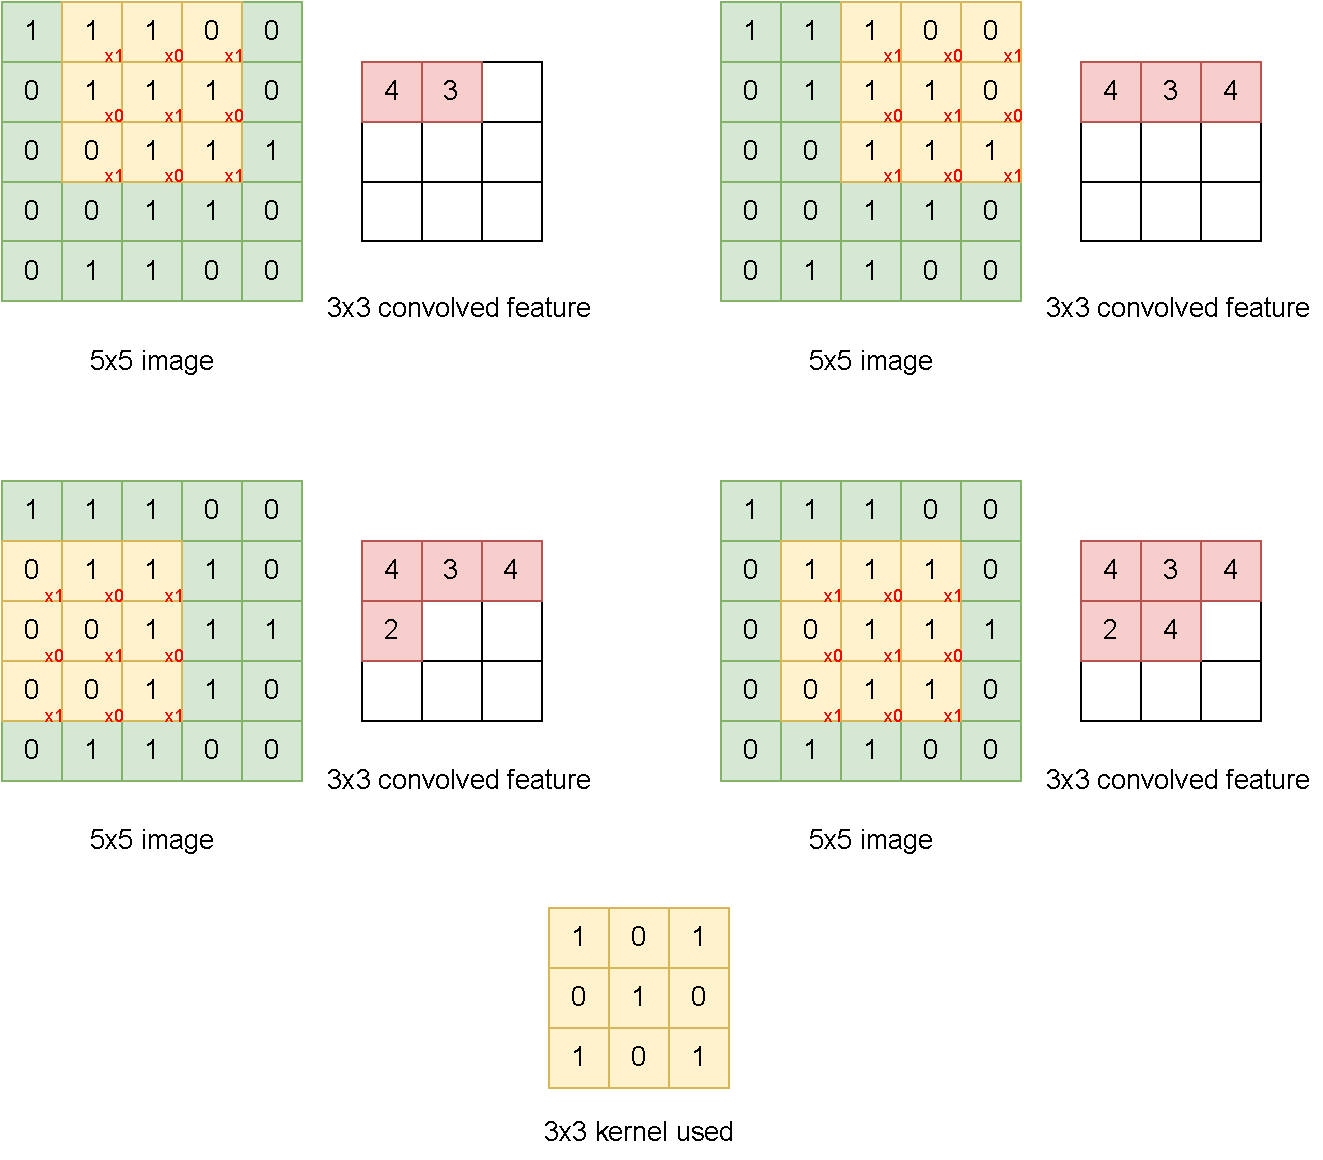
\includegraphics[width=\textwidth]{mlbasics/convolution.pdf}
  \caption[Convolution steps example]{Four example steps during a convolution. A 3x3 window (yellow) containing the kernel values is sliding on an 5x5 image (green) and contructs a 3x3 convolved feature result (red) by an element-wise multiplication.}
  \label{fig:convolution}
\end{figure}

After a convolution, a pooling is performed. The pooling will reduce the dimensionality of the image, and extract the most dominant features that are invariant under translation and rotation. The pooling also uses sliding windows over the convolved image, that will output a specific characteristic depending on the type of pooling. The two most used poolings are the \emph{max pooling}, which extracts the maximal value in the kernel, or the \emph{average pooling} that extracts the average value of all values in the kernel. In case of CNN, the max pooling is typically prefered. Figure~\ref{fig:pooling} shows how the max and average pooling are performed.

\begin{figure}[t!]
  \centering
  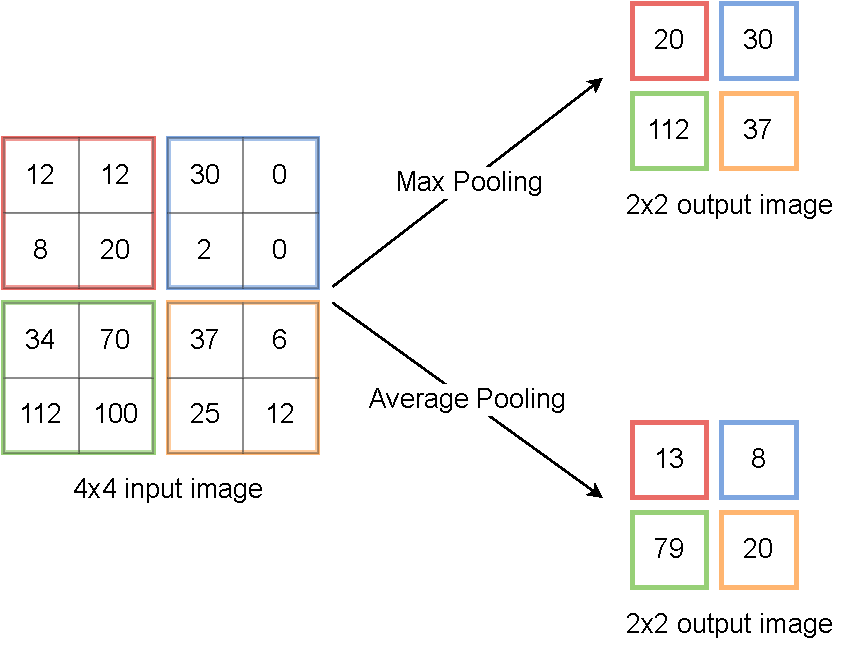
\includegraphics[width=0.62\textwidth]{mlbasics/pooling.pdf}
  \caption[Two of the main types of pooling]{Two of the main types of pooling. Here, a 2x2 kernel is used. The max pooling extracts the maximal value of the kernel, while the average pooling extracts the average of all values within the kernel.}
  \label{fig:pooling}
\end{figure}


\section{Computer aided diagnosis tasks}
\label{sec:tasks}
In the last decades with machine learning and artificial intelligence coming more and more popular and powerful, improvements have been made in the medical field too. With the possibility to use computers to analyze several types of images for many purpose, medical images can be analyzed as well. Techniques can help radiologists in their work, as a second opinion or to detect primary signs of cancer that humans can miss. These techniques are called \emph{Computer Aided Diagnosis} (CAD) systems~\cite{doi_computer-aided_2007}. With the development of deep learning, CAD systems become more and more precise and powerful, by using convolutional neural networks to analyze medical images and perform different tasks, such as classification, localization and segmentation.

\subsection{Classification}
Classification is the task to partition images depending on their characteristics (features). Classification can be binary, i.e. with only two classes, or multi-class. CAD systems can perform this task for example to classify images in a binary manner: The positive class regroups images containing one or more malignant tumors, while the negative class contains images having no malignant masses. The CNN of a CAD system can be trained using supervised learning, but it requires ground truth medical diagnosis. The medical images are the inputs of the network, while the medical diagnoses (true or false) are the labels. By feeding a significant amout of data, the CNN is train and can output a probability that an image contains a malignant tumor. The classification task performed by CAD systems can help radiologists to detect primarily stages of cancer.

\subsection{Localization}
Localization is the task to points the position of an object in an image. In the medical field, a precise location of a malignant tumor is required when doctors are ablating (removing) it. CAD systems can also perform localization: given a medical image in input, they can tell a position where they find a malignant tumor. When training in a supervised learning manner, CAD systems need images as inputs but also ground truth positions (as coordinates for example) of malignant tumors within the image as labels. Finally, an overlay can for example display the location of the tumor outputed by the CAD system.

\subsection{Segmentation}
\label{sec:cadsegtask}
In the medical field, \emph{segmentation} is the process to delimit or contour a specific body part. On one hand, CAD systems can segment organs: for example, \citet{litjens_evaluation_2014} analyzed the results of the 2012 \emph{Prostate MR Image Segmentation} (PROMISE12) challenge organized by the Medical Image Computing and Computer Assisted Intervention society (MICCAI)\footnote{\url{http://www.miccai.org/}}. The goal of this challenge was to develop CAD systems that can perform the segmentation of the prostate, given MRIs of the prostate as inputs. On the other hand, CAD systems can segment malignant tumors: for example, \citet{wang_transbts_2021} develop a CAD system capable of segmenting brain tumors. CAD systems can do segmentation in two or three dimensions. Like classification and localization, segmentation can also be trained with supervised learning. The inputs are the medical images, and the labels are the so called \emph{segmentation masks}. These masks are monochrome (binary) images that have the same size as the input image. Each pixel of the segmentation mask corresponds to a pixel in the medical image. If the pixel is black, the malignant tumor is not present in that position, while if the pixel is white, the tumor is present. Figure~\ref{fig:segmaskimg} illustrates an example of a medical image (input) in~\ref{fig:segmaskimg1} with its corresponding segmentation mask (label) in~\ref{fig:segmaskimg2}, and both are display in a same image in~\ref{fig:segmaskimg3}, where a malignant tumor is colored in red.

\begin{figure}[t!]
     \centering
     \begin{subfigure}[b]{0.32\textwidth}
         \centering
         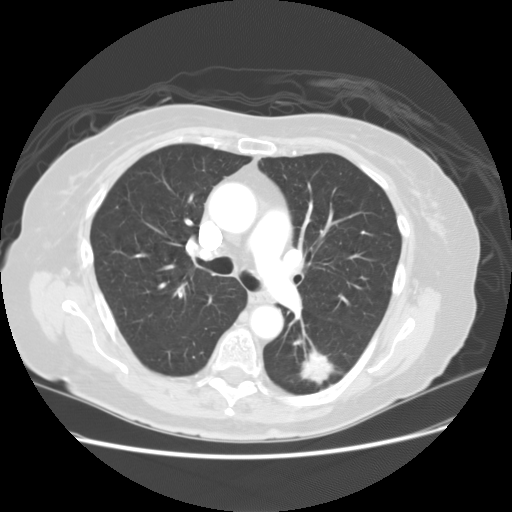
\includegraphics[width=\textwidth]{medicalcontext/medimg.png}
         \caption{CT scan of the lungs}
         \label{fig:segmaskimg1}
     \end{subfigure}
     \hfill
     \begin{subfigure}[b]{0.32\textwidth}
         \centering
         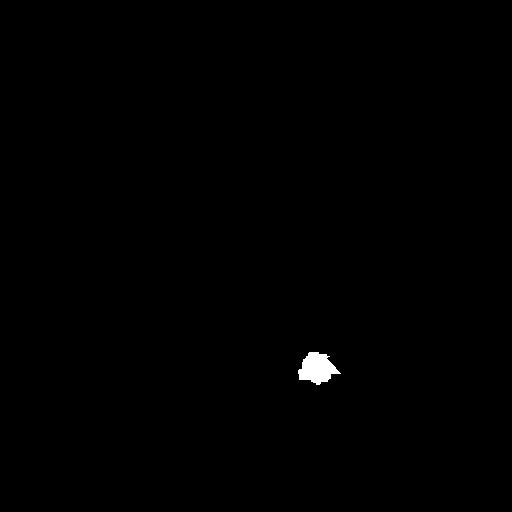
\includegraphics[width=\textwidth]{medicalcontext/segmask.png}
         \caption{Segmentation mask}
         \label{fig:segmaskimg2}
     \end{subfigure}
     \hfill
     \begin{subfigure}[b]{0.32\textwidth}
         \centering
         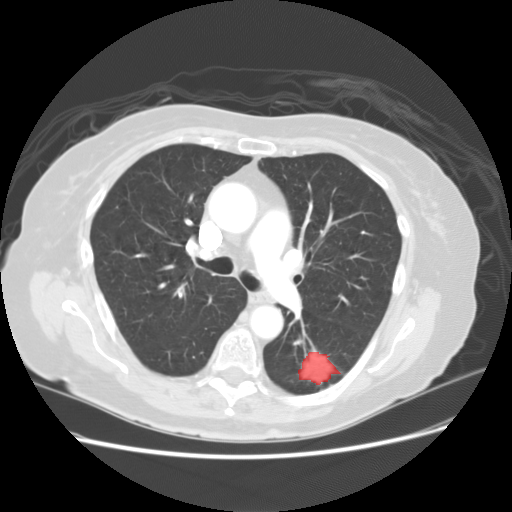
\includegraphics[width=\textwidth]{medicalcontext/imgmask.png}
         \caption{Tumor colored in red}
         \label{fig:segmaskimg3}
     \end{subfigure}
        \caption[Computed tomography scan of the lungs and its segmentation mask]{Example image of a computed tomography scan of the lungs and its segmentation mask from the LIDC-IDRI dataset~\cite{armato_data_2015}. The detected malignant tumor is colored in red in the right image.}
        \label{fig:segmaskimg}
\end{figure}


\section{Hydra framework}
As stated in the motivation of this work, the main goal of this project is to develop a CAD system with the collaboration of the H-FR. This CAD system can help the radiologists in their work. At this time, the Hydra project has been first trained to do tumor detection on the prostate, the lungs and the brain. The name Hydra comes from the shape of the network. It is composed of a body with many heads, like the mythical creature: The body is the feature extractor of the network, i.e. the part where the image is analyzed and convolved and is the same for all type of organs, because tumors share common characteristics. The multiple heads are a set of decision makers returning the probability or not to find a tumor. Each head is specialized for a precise organ. Currently, there is one head for the prostate, one for the lungs and one for the brain. When predicting a specific organ, the body of Hydra will be taken, and the head for the specific organ will be attached. In that way, the feature extraction is general enough to have a good intuition for the decision, and the decision maker is specialized enough to give the right decision for a specific organ. Figure~\ref{fig:hydra} shows the generic form of the Hydra CNN model.
\begin{figure}[t!]
  \centering
  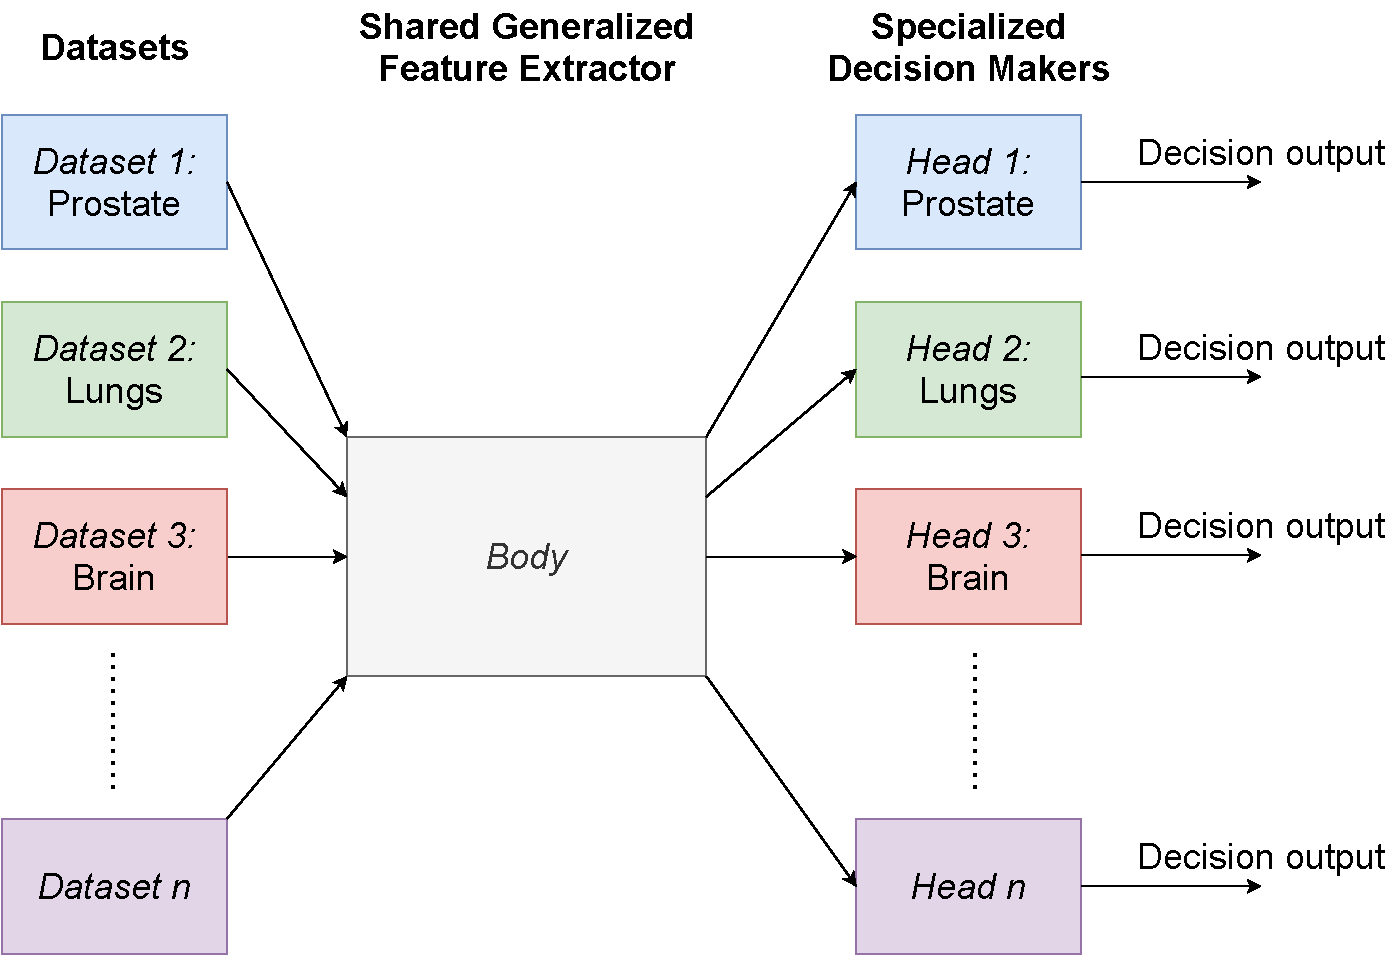
\includegraphics[width=\textwidth]{mlbasics/hydra.pdf}
  \caption[Hydra generic model]{Generic Hydra model. The body is a feature extractor and is common for all type of organs. The model has then many heads that are the decision makers, each head being specialized for one specific organ. The input dataset enters the network first in the shared feature extractor (the body), and goes to the specialized decision maker attached depending on the organ (the head). The decision goes out of the head.}
  \label{fig:hydra}
\end{figure}

This type of architecture avoids the problem of publicly available medical data scarcity stated in the Section~\ref{sec:deeplearning}. It has two advantages:

\vbox{
  \begin{enumerate}
    \item Hydra can learn features from tumors for any organs. Even if data is sparse for a new organ, Hydra uses what it has previously learned from other organs to extract features. In that way, the data used to train the feature extractor is augmented, by aggregating data of any organs. The feature extraction is then generalized.
    \item Each decision maker of Hydra is specialized only for one specific organ. Thus, the heads do not need a lot of data to be train. The scarsity of the data for an organ avoids the generalization of the heads, that could lead to incorrect predictions.
  \end{enumerate}}

The current convolutional neural network model used for Hydra is based on the VGG-16 model architecture~\cite{simonyan_very_2015}, where 16 is the number of layers in the model. The Hydra model contains 9 convolutional layers separated in 3 convolutional blocks of 5 layers each, and 4 fully connected layers at the end. The activation function used after the convolutions is the ELU~\eqref{eq:elu} (see Section~\ref{sec:sl}). Dropout layers are used to prevent overfitting, as training large neural network on relatively small training datasets could overfit the training dataset. To avoid that, dropout layers skip or ignore randomly some neuron's inputs and outputs during the process. This has the effect to preventing the neurons to co-adapt themselves too much during the training~\cite{srivastava_dropout_2014}. Figure~\ref{fig:hydralayers} shows the current full model Hydra with its separated blocks.
\begin{figure}[t!]
  \centering
  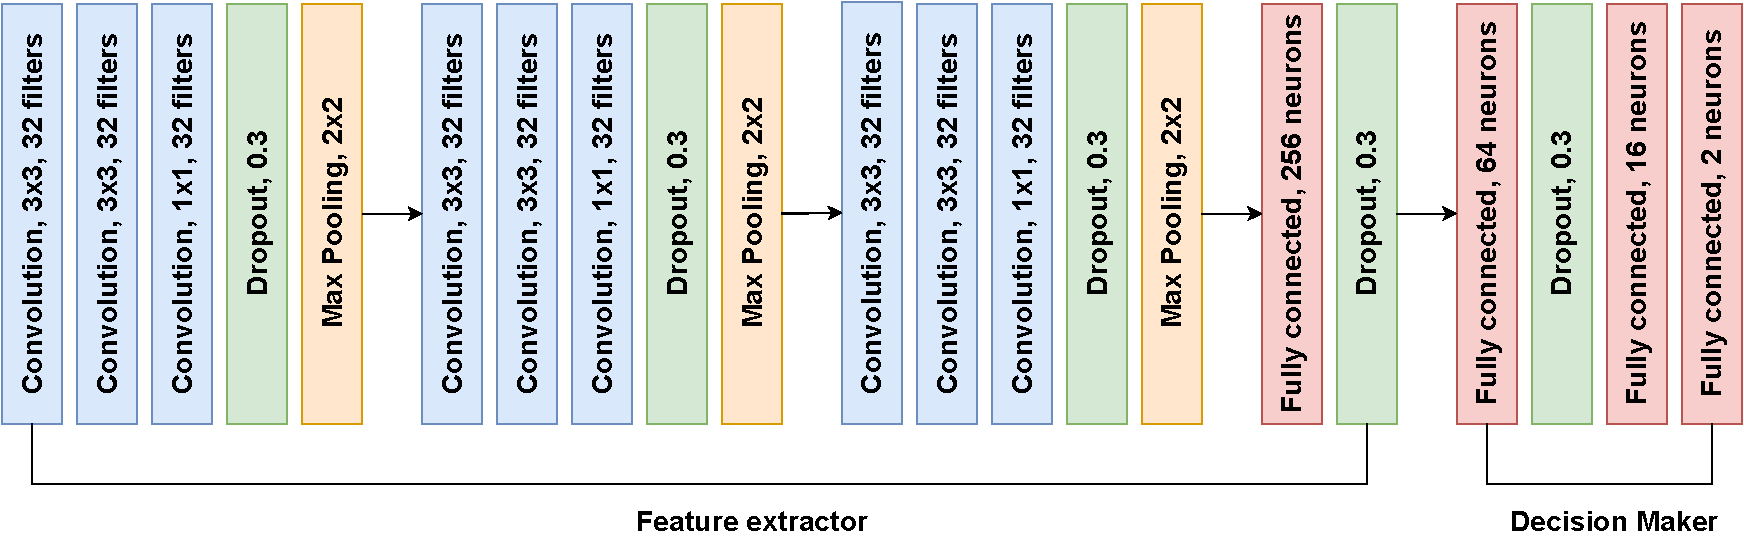
\includegraphics[width=\textwidth]{mlbasics/hydralayers.pdf}
  \caption[Hydra layers]{Full Hydra model, with its layers. The feature extractor is composed of 3 blocks of convolutions ending by a dropout and a max pooling layer. The decision maker is a block of fully connected layers.}
  \label{fig:hydralayers}
\end{figure}
